\documentclass[journal]{IEEEtran}

\usepackage{cite}
\usepackage{amsmath,amssymb,amsfonts}
\usepackage{graphicx}
\usepackage{textcomp}
\usepackage{booktabs}
\usepackage{xcolor}
\usepackage{array}
\graphicspath{{figures/}{../figures/}}

\newcommand{\Pbase}{P_{\mathrm{base}}}
\newcommand{\Estar}{E^{\star}}

\begin{document}

\title{Energy Allocation Between Computation and Wi-Fi Transmission in TinyML Federated Learning: A Measured Crossover}

\author{
\IEEEauthorblockN{Md Abdus Shakur Siam\IEEEauthorrefmark{1} and Farag Azzedin\IEEEauthorrefmark{2}\thanks{Corresponding author: Farag Azzedin.}}
\IEEEauthorblockA{\IEEEauthorrefmark{1}Department of Electrical and Electronic Engineering, Bangladesh University of Engineering and Technology (BUET), Dhaka, Bangladesh \\
abdusshakursiam@gmail.com}
\IEEEauthorblockA{\IEEEauthorrefmark{2}Department of Information and Computer Science, King Fahd University of Petroleum and Minerals (KFUPM), Dhahran, Saudi Arabia}
}

\markboth{IEEE Transactions on Machine Learning in Communications and Networking}%
{Siam and Azzedin: Energy Allocation Between Computation and Wi-Fi Transmission in TinyML Federated Learning}

\maketitle

\begin{abstract}
Most work on wireless federated learning (FL) assumes that sending data over the radio costs far more energy than computing on the device. We test this assumption on a small microcontroller. An ESP32-S3 trains the last layer of a frozen keyword-spotting network and exchanges $3{,}120$-byte model updates over 2.4\,GHz Wi-Fi. An independent INA238 power monitor samples the supply at 1\,kHz, and GPIO markers separate computing from communication. To our knowledge, this is the first physically instrumented measurement of the computation and communication energy crossover for FL over Wi-Fi. A main campaign of 60 runs covers $E\in\{1,2,5,8,10,20\}$ local epochs. Computation costs $1.00$\,mJ per epoch and has no detectable constant term. Communication costs $9.7$\,mJ per client turn, with no clear trend in $E$. The two are equal at $E^\star\approx9.7$ epochs. A second session of 15 runs at the same setting gave $7.4$\,mJ and $E^\star\approx7.4$, so the crossover moves with the radio conditions. A further 45-run test shows that starting training right after a radio burst adds about $0.5$\,mJ to the training energy. A $60$\,ms pause removes it. Five analytical models, including Shannon-capacity and switching-energy models, miss these energies or the crossover by large margins. The one that uses datasheet currents lands within about $10\%$ at its nominal point, but its range is wide. The board also draws $561$\,mW just by being awake. If the device sleeps between rounds, our model moves the crossover to about $11$ to $19$ epochs. The sleep powers used there are assumed values, and so is the effect of channel contention. We end with design guidelines and a clear list of what was measured and what was assumed.
\end{abstract}

\begin{IEEEkeywords}
Federated learning, TinyML, energy efficiency, computation and communication trade-off, Wi-Fi, duty cycling, power measurement.
\end{IEEEkeywords}

\section{Introduction}
\IEEEPARstart{F}{ederated} learning (FL) lets wireless devices train a shared model without sending their raw data~\cite{mcmahan2017communication}. On smartphones, the uplink is the scarce resource. So the usual advice is to run more local epochs $E$ between rounds, which means fewer rounds and less traffic. Many wireless FL papers follow this advice. They allocate bandwidth, transmit power and local computation under analytical models~\cite{zhou2022joint,chen2022federated,zhao2023energy,pham2022energy,ren2022toward,fan2024uavenabled,ju2024befl}. Others compress or quantize the updates~\cite{pan2025rfcsc,xiao2026communication,wang2022communication,paragliola2022evaluation}, or study energy use in IoT settings~\cite{tekin2023energy,sabovic2025energy}. These models usually describe transmission with Shannon capacity and computation with switching energy proportional to $\kappa f^2 C$.

Microcontrollers (MCUs) change the picture. An MCU trains on the same battery that feeds its radio. It has no accelerator, so training is slow. It also draws a lot of power just by staying awake, and the common models have no term for that. The literature does not agree. Some studies find that training dominates~\cite{ficco2024federated,rupaak2026quantifying}. Others, using low-rate radios, find that transfers dominate~\cite{gimenez2023embedded,sanchez2025enhancing,singh2025federated}. These studies use different radios, models and accounting. So they cannot say where the boundary lies on one platform. To our knowledge, none of them locates it with an independent power instrument on a Wi-Fi FL loop.

This paper takes a wireless system design view. A device has a fixed energy budget. It can spend that budget on computing (more local epochs) or on transmitting (more rounds). We ask three questions. At what $E$ does the energy of computing in one turn match the energy of communicating? How does that point move when the radio sleeps between rounds or when the channel is busy? What does it mean for the rounds and airtime that an FL job uses?

Our contributions are as follows.
\begin{enumerate}
\item We measure the energy of computation and communication per client turn on an ESP32-S3 over Wi-Fi. We use a separate power monitor and a fixed protocol with a randomized run order. The main campaign has six values of $E$ and ten repetitions each. Computation grows linearly with $E$. Communication stays about flat. The crossover is near $9.7$ epochs in the main campaign and near $7.4$ in a second session.
\item We run a 45-run test that isolates the post-communication radio tail. It shows how much training energy a burst leaves behind, and how a short pause removes it.
\item We derive a closed-form crossover that includes sleep power and a contention factor. We evaluate it with clearly labeled assumed values.
\item We show how five common analytical models miss the measured energies and the crossover, and we explain why.
\item We break one client turn into protocol phases and link convergence to rounds, bytes and airtime. We separate the hardware crossover $\Estar$ from the learning optimum $E_{\mathrm{opt}}$, and we state the status of every number.
\end{enumerate}
Instrumentation details are in Appendix~A. The status of each result and the corrections to our earlier material are in Appendix~B.

\section{System Model}
\subsection{Protocol and Energy Accounting}
A client holds $D_k$ local audio clips. In each turn it fetches a configuration, downloads the global model head ($3{,}120$\,B), runs $E$ epochs of mini-batch SGD with batch size $B=16$, and uploads the updated head ($3{,}120$\,B). The host averages the uploads with FedAvg.

We use two kinds of energy accounting, because the choice changes the answer. \emph{Marginal energy} is the energy above the awake baseline power $\Pbase$. It shows what computing and communicating add. For one turn,
\begin{align}
\Delta E_{\mathrm{active}}(E)&=\Delta E_{\mathrm{comp}}(E)+\Delta E_{\mathrm{comm}},\\
\Delta E_{\mathrm{comp}}(E)&=\alpha E+c_0 .
\label{eq:marginal}
\end{align}
Here $\Delta E_{\mathrm{comm}}$ does not depend on $E$. It covers the model download and the model upload. The configuration request is not part of it, and Section~\ref{sec:crossover} shows what changes if it is counted. \emph{Gross awake energy} also counts $\Pbase$ over the active time. This time is
\begin{equation}
T_{\mathrm{active}}(E)=T_{\mathrm{comm}}+t_{\mathrm{ep}}E,
\end{equation}
where $t_{\mathrm{ep}}$ is the time of one epoch. If the device sleeps for the rest of a period $T_r$ at power $P_s$, and pays a wake-up energy $E_{\mathrm{wake}}$, the energy of one turn is
\begin{multline}
E_{\mathrm{turn}}(E,T_r)=\Pbase T_{\mathrm{active}}(E)+\Delta E_{\mathrm{active}}(E)\\
+P_s\bigl(T_r-T_{\mathrm{active}}(E)\bigr)+E_{\mathrm{wake}} .
\label{eq:eturn}
\end{multline}
Our main metric is the energy of one client turn. The energy of a round with $K$ clients is $K\,E_{\mathrm{turn}}$.

\subsection{Crossover and Design Problem}
The crossover $\Estar$ is the number of epochs at which computation and communication cost the same. In standby this means $\Delta E_{\mathrm{comp}}(\Estar)=\Delta E_{\mathrm{comm}}$. When the device sleeps between turns, the awake baseline during the active window adds to both terms. The crossover then becomes
\begin{equation}
\Estar(P_s)=\frac{(\Pbase-P_s)\,T_{\mathrm{comm}}+\Delta E_{\mathrm{comm}}-c_0}{(\Pbase-P_s)\,t_{\mathrm{ep}}+\alpha}.
\label{eq:unified}
\end{equation}
The design problem is to choose $E$ so that the energy to reach a target accuracy is smallest:
\begin{equation}
E_{\mathrm{opt}}=\arg\min_{E}\; R(E)\,E_{\mathrm{turn}}(E,T_r),
\label{eq:eopt}
\end{equation}
where $R(E)$ is the number of rounds needed. The value $\Estar$ belongs to the hardware and the protocol. The value $E_{\mathrm{opt}}$ also depends on the data, the learning rate and the target. They are different quantities. We do not use one to confirm the other.

\subsection{Contention}
When other devices use the channel, each exchange takes longer. We model this with an airtime factor $\kappa_c\ge1$ on the communication energy: $\Delta E_{\mathrm{comm}}(\kappa_c)=\kappa_c\,\Delta E_{\mathrm{comm}}$. This is a modeling device. We did not measure $\kappa_c$.

\section{Analytical Baselines}
\label{sec:baselines}
We test five models that the wireless FL literature often uses. We take their parameters from the ranges in the cited works.
\begin{itemize}
\item \textbf{Shannon capacity.} The communication energy is $P_{\mathrm{tx}}\cdot 8M/\bigl(B\log_2(1+\mathrm{SNR})\bigr)$. We use $B$ from 20 to 40\,MHz, SNR from 10 to 30\,dB~\cite{chen2022federated,zhao2023energy}, $P_{\mathrm{tx}}$ from 100 to 200\,mW~\cite{espressif_esp32s3_datasheet}, and $M=2\times3120$\,B.
\item \textbf{Switching energy.} The compute energy per epoch is $\kappa f^2 C$~\cite{zhou2022joint,pham2022energy,ren2022toward}, with $f=240$\,MHz and $\kappa$ from $10^{-28}$ to $10^{-27}$.
\item \textbf{Combined.} The crossover is the Shannon communication energy divided by the switching compute energy.
\item \textbf{Datasheet currents.} We multiply the datasheet transmit, receive and CPU currents~\cite{espressif_esp32s3_datasheet} by assumed durations at 3.3\,V.
\item \textbf{Communication dominant.} Communication always costs much more than computation, so $\Estar\gg100$~\cite{mcmahan2017communication}.
\end{itemize}
Table~\ref{tab:mismatch} compares them with our main campaign from Section~\ref{sec:results}. Errors are relative to the measured $\Delta E_{\mathrm{comm}}=9.75$\,mJ, the measured $\alpha=1.002$\,mJ per epoch and $\Estar=9.74$.

\begin{table*}[t]
\centering
\caption{How analytical models miss the measured energies and crossover. Nominal values use the parameters named in the text. Ranges sweep the stated bounds. Errors are relative to the main campaign.}
\label{tab:mismatch}
\scriptsize
\setlength{\tabcolsep}{3pt}
\begin{tabular}{p{1.9cm}cccp{2.0cm}p{1.9cm}p{3.5cm}}
\toprule
Model & $\Delta E_{\mathrm{comm}}$ (mJ/turn) & $\Delta E_{\mathrm{comp}}$ (mJ/epoch) & $\Estar$ (epochs) & Error & Direction & What the model leaves out \\
\midrule
Shannon capacity & 0.056 [0.013, 0.144] & n/a & n/a & $-99.4\%$ (comm.) & Too low & MAC and CSMA overhead, headers, HTTP exchange, analog radio draw \\
Switching energy & n/a & 0.053 [0.011, 0.106] & n/a & $-94.7\%$ (comp.) & Too low & Memory stalls, SRAM and flash access, leakage \\
Combined & 0.056 & 0.053 & 1.07 [0.12, 13.6] & $-89.0\%$ ($\Estar$) & Too low, very wide range & Both of the above \\
Datasheet currents & 10.73 [6.75, 16.25] & 1.012 [0.77, 1.23] & 10.6 [5.5, 21.2] & $+10.1\%$, $+1.0\%$, $+8.8\%$ & Within about $10\%$ at the nominal point, wide range & Baseline draw, regulator loss, assumed burst times \\
Communication dominant & $>100$ & $<0.5$ & $\gg100$ (nominal 500) & about $+5000\%$ ($\Estar$) & Far too high & Ignores that compute reaches parity near 10 epochs \\
\midrule
\textbf{Measured (this work)} & \textbf{9.75} & \textbf{1.002} & \textbf{9.74} (A), \textbf{10.24} (B) & n/a & n/a & INA238, 5\,V rail, $N=60$ \\
\bottomrule
\end{tabular}
\end{table*}

The models fail in different ways. The first three predict energies that are $95\%$ to $99\%$ too low and a crossover that is very uncertain. The communication-dominant premise puts the crossover about $51$ times too far out. A designer who trusted it would pick the wrong operating point. The datasheet model lands within $10\%$ at its nominal point. We do not read this as proof that the model is right. It assumes the burst durations, and its range for $\Estar$ spans a factor of four. It also has no term for the $561$\,mW that the board draws while awake, which is the largest energy in the system. Against the second session (Section~\ref{sec:crossover}), the datasheet communication energy would be $46\%$ too high.

\section{Testbed and Method}
\label{sec:method}
\begin{figure}[t]
\centering
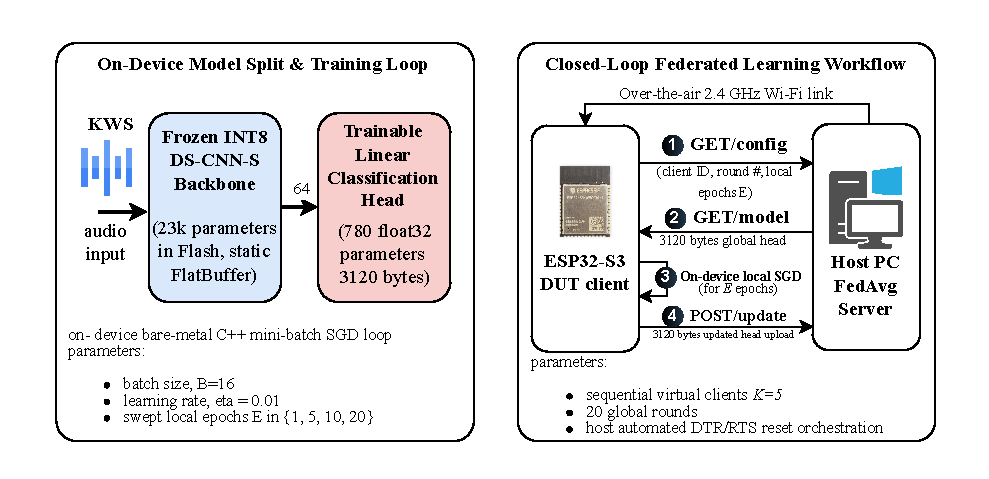
\includegraphics[width=\linewidth]{pipeline.drawio.pdf}
\caption{Testbed. The ESP32-S3 device under test holds a frozen INT8 backbone and a trainable float32 head. An independent INA238 logger measures its supply power. A host runs FedAvg.}
\label{fig:pipeline}
\end{figure}

\subsection{Model Split}
The task is 12-class keyword spotting on Google Speech Commands v2. A frozen INT8 DS-CNN-S backbone with $23{,}552$ parameters produces a 64-dimensional embedding. Training the whole network would not fit in the $512$\,KiB of SRAM. So the device trains only the float32 linear head, which has $64\times12+12=780$ parameters ($3{,}120$\,B) and runs SGD in bare-metal C++. Only this head is sent over the air. The $K$ federated clients in our experiments are virtual. One physical device plays all of them. Each virtual client holds 100 clips, the learning rate is $0.01$, and the batch size is 16.

\subsection{Measurement}
The device under test is an ESP32-S3 with two Xtensa LX7 cores at 240\,MHz and an 802.11 b/g/n radio. A TI INA238 with a $15$\,m$\Omega$ ($1\%$) high-side shunt sits in the supply line. A second ESP32-S3 reads it at 1\,kHz and streams the samples at 921{,}600 baud. The device raises GPIO markers during training and during HTTP exchanges, and a 3-bit phase bus labels sub-phases. Every sample is therefore tagged as train, communicate or idle. Energy is the time integral of power. The supply is 5\,V DC on the board input, which feeds the on-board 3.3\,V regulator. Appendix~A gives the wiring and isolation steps.

All 105 runs use one firmware build, one board pair, one access point and fixed cables. The access point is a phone hotspot on channel 6, $0.5$\,m from the board. The signal strength was $-40$ to $-41$\,dBm at the start and end of every run. Each run has 30\,s of idle before the turn and 30\,s after it. The baseline power of a run is the median power in the window from 5\,s to 25\,s of each idle period, averaged over the two periods. Energy above baseline is the sum of $(P-P_{\mathrm{base}})\,\Delta t$ over the samples of a phase. A run passes only if it has no dropped samples, strictly increasing timestamps, the right number of markers, and a baseline that drifts by less than $2\%$ between the two idle periods. A failed attempt is kept and repeated. Twenty attempts failed, mostly because the training marker never appeared. No sample was repaired or interpolated.

Two campaigns follow. The \emph{main campaign} has 60 runs, with $E\in\{1,2,5,8,10,20\}$ and ten repetitions each. A $60$\,ms pause separates the phases of a turn. The \emph{tail test} has 45 runs, with $E\in\{1,5,20\}$, pauses of $0$, $60$ and $200$\,ms, and five repetitions per cell. The run order was randomized within each campaign.

\subsection{Power Profile}
\begin{figure*}[t]
\centering
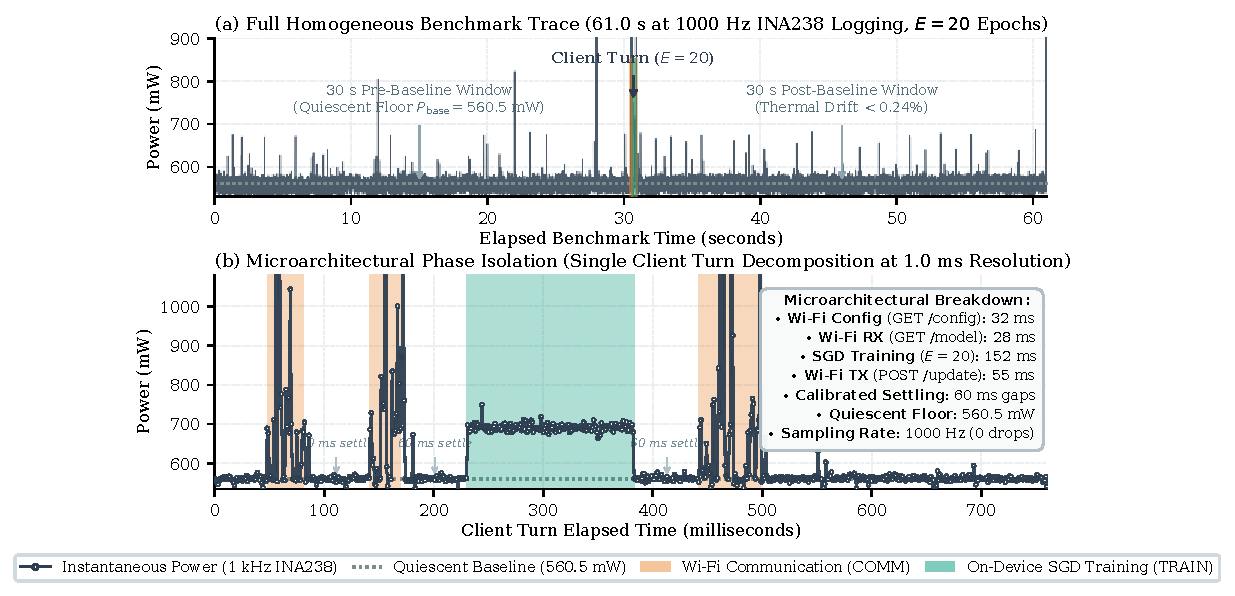
\includegraphics[width=0.8\textwidth]{fig1_power_time_series.pdf}
\caption{Power trace of one main-campaign run ($E=20$) at 1\,kHz. (a) The full 61\,s run, with 30\,s of idle before and after the turn. (b) One client turn: configuration request, model download, SGD, model upload and the $60$\,ms pauses between them.}
\label{fig:power}
\end{figure*}
Figure~\ref{fig:power} shows one run of the main campaign. With modem sleep off, the awake and idle board draws $\Pbase=561.1\pm1.8$\,mW over the 105 runs of this campaign. The baseline of single runs ranges from $557.8$ to $569.7$\,mW. In the run shown, the baseline is $560.5$\,mW. The SGD plateau is $691.5$\,mW, which is $131$\,mW above baseline, and it lasts $152$\,ms. Across the campaign, one epoch takes $7.58$\,ms and costs $1.00$\,mJ above baseline, which is $132$\,mW. Single samples in the radio phases reach about $1$\,W. The $60$\,ms pauses let the radio tail fall before training starts (Section~\ref{sec:tail}).

\section{Measured Crossover}
\label{sec:results}
\subsection{Energy per Turn}
Table~\ref{tab:energy} gives the measured energy per client turn in the main campaign. Computation grows almost linearly with $E$, and its spread is small. Communication varies from $8.6$ to $11.9$\,mJ with no clear trend. A straight-line fit of communication energy on $E$ has a slope of $0.08\pm0.09$\,mJ per epoch.

\begin{table}[t]
\centering
\caption{Measured marginal energy per client turn in the main campaign ($N=10$ per regime). Values are the mean $\pm$ the standard deviation. The ratio is the mean computation energy over the mean communication energy.}
\label{tab:energy}
\scriptsize
\setlength{\tabcolsep}{3pt}
\begin{tabular}{cccccc}
\toprule
$E$ & $T_{\mathrm{train}}$ (ms) & $\Delta E_{\mathrm{comp}}$ (mJ) & $\Delta E_{\mathrm{comm}}$ (mJ) & Median comm. & Ratio \\
\midrule
1  & $7.5\pm0.5$ & $0.99\pm0.06$ & $8.5\pm3.2$ & 7.5 & 0.12 \\
2  & $15.1\pm0.3$ & $2.00\pm0.06$ & $9.4\pm2.9$ & 9.0 & 0.21 \\
5  & $37.9\pm0.3$ & $5.01\pm0.10$ & $10.6\pm6.9$ & 8.5 & 0.47 \\
8  & $60.7\pm0.5$ & $8.01\pm0.19$ & $11.3\pm5.0$ & 9.6 & 0.71 \\
10 & $75.8\pm0.4$ & $9.98\pm0.25$ & $7.9\pm2.2$ & 7.5 & 1.27 \\
20 & $151.6\pm0.5$ & $20.04\pm0.37$ & $10.8\pm4.3$ & 11.1 & 1.86 \\
\bottomrule
\end{tabular}
\end{table}

A least-squares fit of the 60 runs gives
\begin{equation}
\Delta E_{\mathrm{comp}}(E)=1.002\,E-0.010\ \mathrm{mJ},\qquad R^2=0.999 .
\end{equation}
The $95\%$ bootstrap interval is $[0.991,1.014]$ for the slope and $[-0.070,+0.049]$ for the intercept. The intercept is therefore zero within about $0.07$\,mJ. The slope matches the product of the plateau power above baseline and the epoch time, $132\,\mathrm{mW}\times7.58\,\mathrm{ms}=1.00$\,mJ. The mean communication energy over the 60 runs is $\Delta E_{\mathrm{comm}}=9.75$\,mJ, with a $95\%$ interval of $[8.77,10.96]$.

\begin{figure}[t]
\centering
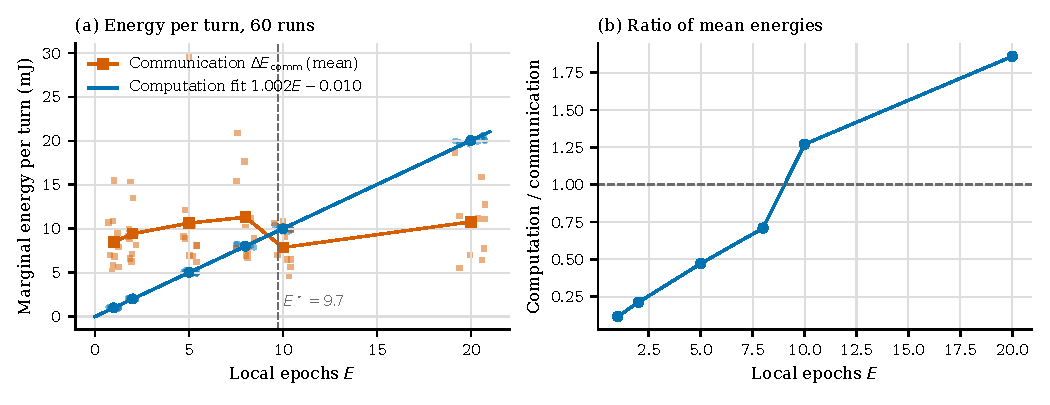
\includegraphics[width=\linewidth]{fig_crossover_v2.pdf}
\caption{Measured marginal energy per client turn in the main campaign. (a) Each point is one run. Computation grows with $E$. Communication is about flat but scattered. The curves meet near $E=10$. (b) The ratio of the mean energies crosses one at the same point.}
\label{fig:crossover}
\end{figure}

\begin{figure}[t]
\centering
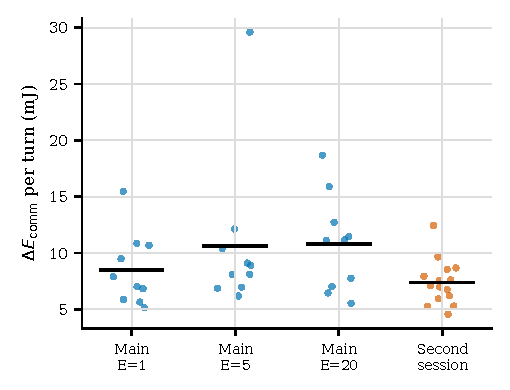
\includegraphics[width=0.85\linewidth]{fig_comm_variation.pdf}
\caption{Communication energy per turn for single runs. The first three groups are from the main campaign. The last group is the second session at the same $60$\,ms setting. Bars mark the means.}
\label{fig:commvar}
\end{figure}

Communication energy scatters much more than computation energy. Its standard deviation is about $2$ to $7$\,mJ, against $0.06$ to $0.4$\,mJ for computation. The cause is the radio exchange. Most exchanges take 85 to 163\,ms (the middle half of all 105 runs), but some stall. In 6 of the 105 runs the exchange took more than $500$\,ms, and the longest took $2.8$\,s. A stall adds energy because the radio stays on. This is why the mean ($9.75$\,mJ) lies above the median ($8.85$\,mJ).

\subsection{Crossover}
\label{sec:crossover}
The crossover is $\Estar=(\Delta E_{\mathrm{comm}}-c_0)/\alpha$. We state it in three ways.
\begin{itemize}
\item \textbf{Version A.} We use the communication energy of the two model exchanges as the markers set it. Then $\Estar=9.74$ epochs, with a $95\%$ bootstrap interval of $[8.79,10.85]$.
\item \textbf{Version B.} We charge a $0.506$\,mJ radio tail to communication. Then $\Estar=10.24$ epochs, with an interval of $[9.30,11.36]$. The tail value comes from an earlier pilot. Section~\ref{sec:tail} measures the tail directly.
\item \textbf{Configuration included.} The configuration request costs $3.4$\,mJ on average. If we count it as communication, $\Estar=13.1$ epochs, with an interval of $[11.9,14.4]$.
\end{itemize}
Below the crossover, communication takes most of the marginal energy. Above it, computation does. At $E=20$, computation is $65\%$ of the marginal energy of a turn.

The main campaign is not the only measurement. The tail test has 15 runs at the same $60$\,ms setting and $E\in\{1,5,20\}$. They give $\Delta E_{\mathrm{comm}}=7.37$\,mJ and $\Estar=7.42$ epochs, with an interval of $[6.54,8.36]$. For the same values of $E$, the main campaign gives $9.97$\,mJ. The difference is $2.6$\,mJ (Welch $t=2.5$, permutation test $p=0.05$). Our earlier pilot campaign, with a different logger setup, gave $7.33$\,mJ and $\Estar=7.4$. We did not log retries or the load of the phone hotspot, so we cannot say why the sessions differ. We can say that the variation between sessions is larger than the effect of the tail in the next subsection. We therefore report the crossover as about $7.5$ to $10$ epochs. The main campaign, which has the most runs, gives the upper end. The computation side is stable: the tail test gives a slope of $0.996$\,mJ per epoch at $60$\,ms, which agrees with $1.002$.

\subsection{The Radio Tail}
\label{sec:tail}
After a radio burst, the power takes a short time to fall back to the baseline. If training starts at once, the end of this tail can land in the training window. The tail test checks this. It compares back-to-back phases ($0$\,ms) with pauses of $60$\,ms and $200$\,ms.

\begin{table}[t]
\centering
\caption{Linear fit of training energy against $E$ for each settling delay. Each row has 15 runs, five each at $E=1$, 5 and 20. Intervals are $95\%$ bootstrap intervals.}
\label{tab:tail}
\scriptsize
\setlength{\tabcolsep}{3pt}
\begin{tabular}{cccc}
\toprule
Delay (ms) & Slope $\alpha$ (mJ/epoch) & Intercept $c_0$ (mJ) & $R^2$ \\
\midrule
0 & 1.020 [0.997, 1.048] & $+0.475$ [0.182, 0.786] & 0.997 \\
60 & 0.996 [0.973, 1.026] & $-0.014$ [$-0.112$, 0.075] & 0.998 \\
200 & 1.006 [0.993, 1.017] & $+0.020$ [$-0.033$, 0.077] & 1.000 \\
\bottomrule
\end{tabular}
\end{table}

\begin{figure}[t]
\centering
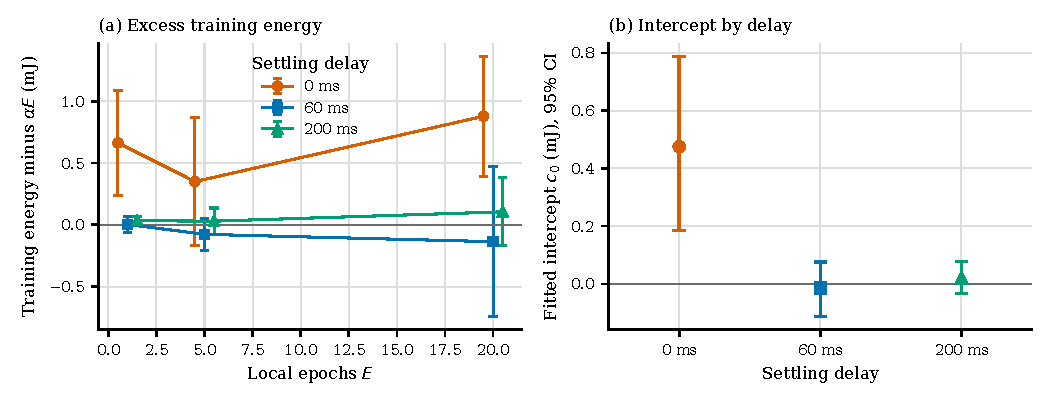
\includegraphics[width=\linewidth]{fig_tail_ab.pdf}
\caption{Tail test. (a) Training energy above the line $\alpha E$, with $\alpha=1.002$, for three settling delays. Bars show one standard deviation. (b) The fitted intercept for each delay, with its $95\%$ interval.}
\label{fig:tailab}
\end{figure}

Table~\ref{tab:tail} and Fig.~\ref{fig:tailab} show the result. With no pause, the intercept is $+0.48$\,mJ. With a $60$\,ms pause it is $-0.01$\,mJ. The difference is $0.49$\,mJ, with a $95\%$ interval of $[0.18,0.82]$. A permutation test that shuffles the delay labels within each $E$ gives $p=0.04$. A pause of $200$\,ms gives the same result as $60$\,ms. Their intercepts differ by $0.03$\,mJ, with an interval of $[-0.07,0.15]$. The evidence is moderate. Each cell has only five runs, and the extra energy at $0$\,ms is not the same for each $E$. It is $0.66$, $0.43$ and $1.02$\,mJ at $E=1$, 5 and 20.

The traces show where the extra energy comes from. Figure~\ref{fig:tailprofile} shows the mean power above baseline in the $60$\,ms pause after each phase. The pause after the model download holds $0.75$\,mJ. The pause after the configuration request holds $0.76$\,mJ, and the pause after the upload holds $0.59$\,mJ. Most of this falls within $20$\,ms. The pause after training holds only $0.11$\,mJ. So a radio burst leaves about $0.6$ to $0.8$\,mJ behind, and a training burst leaves little. In the five back-to-back runs at $E=20$, the first $10$\,ms of training draw on average $171$\,mW above baseline. Training draws $129$ to $133$\,mW above baseline when it starts after a pause. These numbers agree with the extra $0.5$ to $1$\,mJ in the fit.

\begin{figure}[t]
\centering
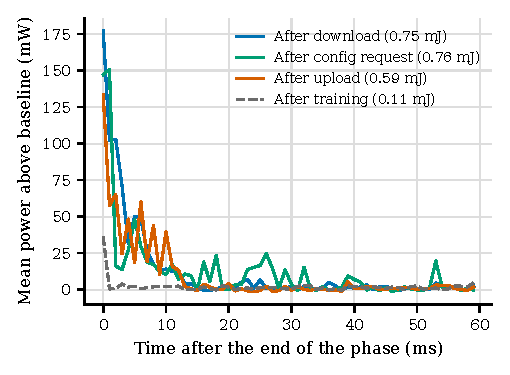
\includegraphics[width=0.9\linewidth]{fig_tail_profile.pdf}
\caption{Mean power above baseline after the end of each phase, taken from the $60$\,ms pauses of 74 runs. The numbers in the legend are the energy in the first $60$\,ms.}
\label{fig:tailprofile}
\end{figure}

Two points follow. First, a measurement that starts training right after a radio burst overstates the compute energy by about $0.5$\,mJ, which is half an epoch at $E=1$. Second, the tail is real communication cost. It is paid after every burst. If both the download tail and the upload tail were charged to communication, the cost would rise by about $1.1$\,mJ and $\Estar$ by about $1.1$ epochs. Version B charges only one tail of $0.506$\,mJ, so it is a lower bound. The pause is a measurement tool. A real firmware may not wait for the tail, and then the tail energy still has to be paid by someone.

\subsection{Link-Layer Breakdown}
\label{sec:linklayer}
The phase bus lets us see where the time of an exchange goes. Table~\ref{tab:linklayer} lists the result for all 105 runs.
\begin{table}[t]
\centering
\caption{Phases of one client turn from the phase bus. Times are the median with the middle half of the runs in brackets, for all 105 runs. Energies are the mean $\pm$ the standard deviation above baseline.}
\label{tab:linklayer}
\scriptsize
\setlength{\tabcolsep}{3pt}
\begin{tabular}{lccc}
\toprule
Phase & Protocol state & Time (ms) & Energy (mJ) \\
\midrule
Config request & HTTP GET of the configuration & 41 [28, 69] & $3.3\pm2.5$ \\
Download & HTTP GET of the model head & 37 [27, 57] & $3.6\pm1.7$ \\
Training & Local SGD ($E$ epochs) & $7.58E$ & $1.00E$ \\
Upload & HTTP POST of the update & 85 [46, 115] & $5.4\pm3.0$ \\
\midrule
Download and upload & & 125 [84, 163] & $9.0\pm3.7$ \\
\bottomrule
\end{tabular}
\end{table}
The payload itself is small. Moving $3{,}120$\,B at an OFDM rate takes less than a millisecond. Even so, the download takes about $37$\,ms and the upload about $85$\,ms. So most of the time goes to the protocol and to the radio, not to the bits. This also explains why the Shannon model fails. The upload costs more than the download because the radio transmits. The configuration request, which carries almost no data, costs as much as the model download. The communication time of a turn is $125$\,ms at the median, with a long tail from stalls. The sleep results below use $T_{\mathrm{comm}}$ from $85$ to $160$\,ms, which is the middle half of the runs.

\section{Sleep and Channel Contention}
\label{sec:sleepcont}
\emph{The sleep powers and wake-up energies in this section are datasheet-style assumptions. We did not measure them on our board. We also did not measure channel contention.} We use them to show how the problem changes, not to claim savings.

\subsection{Sleep Moves the Crossover}
In standby, the awake baseline is paid whether or not the device works, so it drops out of the marginal comparison. If the device sleeps between turns, the baseline during the active window becomes a real cost. A longer exchange costs more, and so does every epoch. One epoch takes $7.58$\,ms at $561$\,mW, which is $4.3$\,mJ. That is more than four times its marginal $1.00$\,mJ. Evaluating Eq.~\eqref{eq:unified} gives Table~\ref{tab:sleep}. The crossover rises from $9.7$ to between $11$ and $19$ epochs as soon as sleep is possible. The choice of sleep state matters little. The value of $T_{\mathrm{comm}}$ matters much more, which is why the stalls in Section~\ref{sec:linklayer} matter for a designer.

\begin{table}[t]
\centering
\caption{Crossover from Eq.~\eqref{eq:unified} and energy per turn at $T_r=60$\,s, using $T_{\mathrm{comm}}=125$\,ms for the energies. The sleep power and wake-up energy are assumed values.}
\label{tab:sleep}
\scriptsize
\setlength{\tabcolsep}{2pt}
\begin{tabular}{lccccccc}
\toprule
State & $P_s$ (mW) & $E_{\mathrm{wake}}$ (mJ) & \multicolumn{2}{c}{$\Estar$ for $T_{\mathrm{comm}}=$} & \multicolumn{3}{c}{$E_{\mathrm{turn}}$ (J)} \\
 & & & 85\,ms & 160\,ms & $E{=}1$ & $E{=}5$ & $E{=}20$ \\
\midrule
Standby & 561.1 & 0 & 9.7 & 9.7 & 33.68 & 33.68 & 33.70 \\
Modem sleep & 100 & 0 & 10.9 & 18.6 & 6.07 & 6.09 & 6.16 \\
Light sleep & 10 & 0.5 & 10.9 & 18.9 & 0.685 & 0.705 & 0.783 \\
Deep sleep & 0.08 & 180 & 10.9 & 18.9 & 0.270 & 0.291 & 0.370 \\
\bottomrule
\end{tabular}
\end{table}

Two points follow even with assumed values. In standby, a 60\,s turn costs about $33.7$\,J whatever $E$ is, so idling dominates. In deep sleep, the same turn costs about $0.3$\,J, and the wake-up energy and the active window dominate. So how much a saved round is worth depends on the sleep regime. That regime is a power-management choice, not a learning hyperparameter.

\subsection{Contention}
With the airtime factor of Section~II-C, the standby crossover is $\Estar(\kappa_c)=(\kappa_c\cdot9.748+0.0098)/1.002$. It gives $9.7$, $14.6$, $19.5$ and $29.2$ for $\kappa_c=1$, $1.5$, $2$ and $3$. The direction is clear. A busy channel lengthens each exchange and pushes the crossover up, so more local work per round pays off. The size of the effect is a hypothesis, because we did not vary the channel load.

\section{Convergence, Rounds and Spectrum Use}
\label{sec:conv}
\subsection{Setup}
Easy tasks let every setting reach the target in one round, which hides the trade-off. We therefore use a harder simulated task. It has $K=20$ clients with $100$ clips each, Dirichlet label skew with $\alpha=0.3$, $10$\,dB acoustic noise and $20$ random seeds. Rounds to the target are fractional, found by linear interpolation. The learning rate is tuned for each $E$ with $\eta\le1.0$. We dropped an earlier run at $\eta=3.0$. Its logits ran from $-54.6$ to $+106.4$ and hit the clipping limit of $\pm50$. This hid divergence and lowered the final accuracy from $79.8\%$ to $76.7\%$. The target is $75\%$ test accuracy. We did not rerun this simulation for the present paper. The rounds $R(E)$ are the earlier results.

\subsection{Rounds, Bytes, Airtime and Energy}
Table~\ref{tab:conv} lists the simulated rounds $R(E)$. The energy columns are computed here. We combine $R(E)$ with the fitted energy model of Eq.~\eqref{eq:marginal} and the main-campaign $\Delta E_{\mathrm{comm}}$, a time $T_{\mathrm{active}}=125+7.58E$\,ms, and, for the last column, the assumed deep-sleep values. One client moves $2\times3{,}120=6{,}240$\,B per round. Traffic and channel accesses to the target therefore scale with $R(E)$. From $E=1$ to $E=20$, the traffic per client falls from about $34$\,kB to $8.7$\,kB. The number of rounds, each with a download and an upload, falls from about $5.4$ to $1.4$.

\begin{table}[t]
\centering
\caption{Energy per client to reach $75\%$ accuracy in the $K=20$ non-IID simulation. Marginal and gross energies use the measured fit. The last column assumes $P_s=0.08$\,mW, $E_{\mathrm{wake}}=180$\,mJ and $T_r=60$\,s.}
\label{tab:conv}
\scriptsize
\setlength{\tabcolsep}{3pt}
\begin{tabular}{cccccc}
\toprule
$E$ & $R(E)$ & Traffic (kB) & Marginal (J) & Gross awake (J) & Deep sleep (J) \\
\midrule
1  & 5.42 & 33.8 & 0.058 & 0.461 & 1.46 \\
2  & 3.75 & 23.4 & 0.044 & 0.339 & 1.03 \\
5  & 2.05 & 12.8 & \textbf{0.030} & \textbf{0.218} & 0.60 \\
8  & 1.82 & 11.4 & 0.032 & 0.222 & 0.56 \\
10 & 1.80 & 11.2 & 0.036 & 0.238 & 0.57 \\
20 & 1.40 & 8.7  & 0.042 & 0.259 & \textbf{0.52} \\
\bottomrule
\end{tabular}
\end{table}

\begin{figure}[t]
\centering
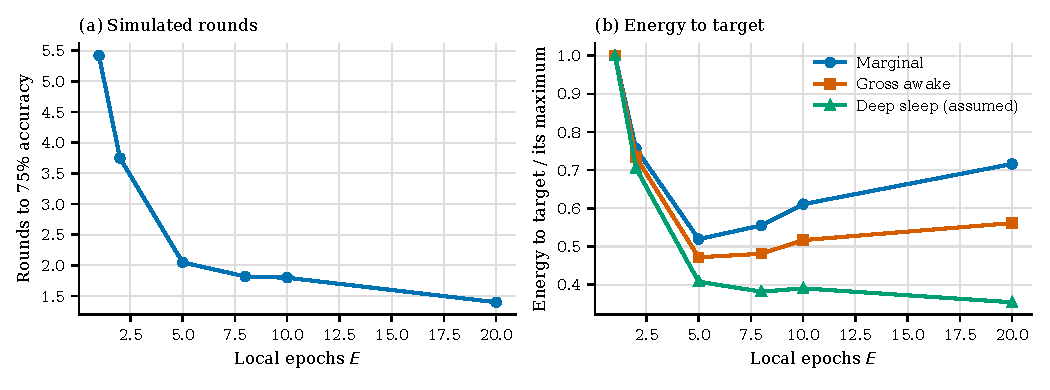
\includegraphics[width=\linewidth]{fig_energy_to_target_v2.pdf}
\caption{(a) Simulated rounds to $75\%$ accuracy. (b) Energy to target for each accounting, each divided by its own maximum.}
\label{fig:conv}
\end{figure}

\subsection{Crossover and Learning Optimum}
The best $E$ depends on how energy is counted. For marginal energy it is $E=5$. For gross awake energy it is also $E=5$, with $E=8$ close behind ($0.218$ and $0.223$\,J). For the assumed deep-sleep model it is $E=20$, the largest value we tested. The hardware crossover is about $10$ in marginal terms and $11$ to $19$ in gross terms with sleep. These numbers differ, and they should. In this task, $R(E)$ stops falling after about $E=5$ to $10$, while compute energy keeps growing. This round floor is probably set by how well clients agree on skewed data. Client drift may add to it, but we did not test that. On an easier task, the same hardware would give a different $E_{\mathrm{opt}}$. So $\Estar$ alone does not decide the best setting. The radio, the sleep schedule and the data all play a part.

\section{Design Guidelines}
\label{sec:guidelines}
\begin{enumerate}
\item \textbf{Do not assume that communication dominates on an MCU.} On this platform the marginal energies match between about $8$ and $10$ epochs. The common choice of $E=5$ to $10$ sits below or near that point, so communication is still the larger marginal term for most of that range. Computation is not negligible.
\item \textbf{Count the cost of being awake.} At $E=1$, the awake baseline over a turn is about $74$\,mJ, while the marginal energy is about $11$\,mJ. Sleep scheduling can matter more than tuning $E$.
\item \textbf{Treat the round period and sleep state as design variables.} In deep sleep, a round is expensive because of the wake-up. In standby it is cheap. Choose $E$ with the sleep model of the deployment, using Eqs.~\eqref{eq:eturn} and~\eqref{eq:eopt}.
\item \textbf{Count protocol overhead, not payload.} The payload takes under a millisecond of airtime, yet an exchange takes tens of milliseconds. Fewer connections or a persistent connection attack the main cost. A smaller payload does not.
\item \textbf{Watch for stalls.} A few exchanges take hundreds of milliseconds or more. They add energy and raise the mean. Time-outs and retry rules matter for the energy budget.
\item \textbf{Leave a gap after a radio burst when you measure compute.} Without it, about $0.5$\,mJ of tail energy lands in the training window. In a deployed system, count that tail as communication.
\item \textbf{Expect contention to favor more local work.} If contention stretches each exchange by $\kappa_c$, the crossover grows about in proportion. This is a hypothesis for now.
\item \textbf{Measure with an independent instrument.} Our earlier accounting had an integration error and a synthetic convergence curve (Appendix~B). An external monitor with hardware markers exposed both.
\end{enumerate}
Other radios fit the same framework if one replaces $\Delta E_{\mathrm{comm}}$ and $T_{\mathrm{comm}}$. A slow low-power wide-area link would push $\Estar$ much higher. A short-range burst radio would pull it lower. This agrees with the split in the literature~\cite{gimenez2023embedded,ficco2024federated}, but we did not measure either radio.

\section{Limitations}
\label{sec:limits}
\begin{itemize}
\item We used one device, one board, one radio, one task and one trainable head. The $K$ clients are virtual.
\item Communication energy varies a lot. The standard deviation is $2$ to $7$\,mJ per regime. The main campaign and the second session differ by $2.6$\,mJ at the same setting, and we cannot explain why. The crossover is therefore a range of about $7.5$ to $10$ epochs.
\item The access point is a phone hotspot. We did not log retries, channel load or the hotspot state.
\item The tail test covers $E=1$, 5 and 20 with five runs per cell. Its main result has $p\approx0.04$. The extra energy at $0$\,ms is not constant across $E$.
\item The three communication windows are integrated against a baseline about $1.6$\,mW lower than the one used for the training window. This raises the reported communication energy by about $0.4$\,mJ per turn and the main-campaign crossover by about $0.4$ epochs (Appendix~A).
\item Sleep power, wake-up energy, contention and payload size were not measured. Their results are model-only.
\item Convergence is simulated and was not rerun for this paper. We did not check bit-level agreement between the device and the simulation. The energy-to-target table combines simulated rounds with measured per-turn energy.
\item The analytical-model parameters come from ranges in the cited works. Other choices change the errors, but not their direction.
\end{itemize}

\section{Conclusion}
On an ESP32-S3 over Wi-Fi, with an independent power monitor, computation costs $1.00$\,mJ per epoch with no detectable constant term. Communication costs $9.7$\,mJ per client turn in a 60-run campaign and $7.4$\,mJ in a second session. The marginal crossover is therefore about $7.5$ to $10$ epochs, and $9.7$ in the larger campaign. A radio burst leaves a tail of about $0.6$ to $0.8$\,mJ. Training that starts right after a burst absorbs part of it, unless a short pause intervenes. Common analytical models miss the energies by $95\%$ to $99\%$, or give a crossover that is far too high or too uncertain. The datasheet model is within about $10\%$ at its nominal point but has a wide range. If the device can sleep between rounds, our model moves the crossover to between $11$ and $19$ epochs. The best number of local epochs then depends on the sleep regime. That is a power-management choice as much as a learning choice. Direct measurements of sleep power, wake-up energy and channel contention would turn the model-based parts of this paper into measured results.

\appendices
\section{Instrumentation Details}
\textbf{Sensing.} An INA238 with a $15$\,m$\Omega$ ($1\%$) shunt sits on the high side of the device supply. The ADC range is $\pm163.84$\,mV, the conversion time is $540$\,\textmu s, and there is no averaging. A second ESP32-S3 reads current and bus voltage at 1\,kHz and sends them over a USB serial link at 921{,}600 baud. Power is $P=V_{\mathrm{bus}}I$. Energy is a sum over $1$\,ms samples between marker edges.

\textbf{Markers.} GPIO~10 marks training and GPIO~11 marks communication. A 3-bit phase bus on GPIO~12, 13 and 14 labels sub-phases and is read by the logger. Each line has a $100$\,k$\Omega$ pull-down resistor.

\textbf{Isolation.} USB power is removed from the device during measurement. A connected host would back-power the board and bypass the shunt. The device, the INA238 and the logger share one ground.

\textbf{Supply.} The bench supply gives $5.0$\,V DC to the board input, which feeds the on-board $3.3$\,V regulator. The multimeter read $5.04$\,V before and after the campaign. The logged bus voltage averaged $5.03$\,V, and it dips during radio and training bursts.

\textbf{Quality gates and rejected runs.} A run passes only if it has zero dropped samples, strictly increasing timestamps, the expected marker count and a baseline drift below $2\%$. The 105 accepted runs had a mean drift of $0.24\%$ and a largest drift of $0.84\%$. Twenty attempts were rejected and repeated, and their traces are kept. Nineteen of them showed no training marker. The bench log blames a serial reset when the port opened and the phone hotspot going to sleep, but we did not test these causes. One attempt had 99 dropped samples and a bad first timestamp. The accepted traces were not edited.

\textbf{Integration of the communication windows.} Energy is the sum of $(P-P_{\mathrm{base}})\cdot1$\,ms over the window, and negative terms are kept. The first version of our analysis pipeline set negative terms to zero in the communication windows. Noise in the baseline then adds a positive bias, because a window with no signal would still sum to more than zero. On idle samples held out from the baseline estimate, this bias is $2.8$\,mW on average. It grows with the window length, so it is largest in the runs with long stalls. The training windows are not affected, because power during training is always above baseline. We therefore report the unclamped sums. They lower the mean communication energy of the main campaign from $10.16$ to $9.75$\,mJ and the crossover from $10.15$ to $9.74$ epochs. We checked this by integrating the raw traces independently. The training energies agree with the pipeline to within $0.005$\,mJ in all 105 runs. The clamped communication sums agree with the first pipeline in 102 of 105 runs to within $0.002$\,mJ, so the difference comes only from the clamping.

\section{Status of Results and Corrections}
\textbf{Corrections to earlier material.}
\begin{itemize}
\item An earlier convergence figure, a ``36\% saving'' and a loss value of $4.82$ came from a synthetic formula, not from training. We do not use them.
\item An earlier table of gross round energies was too low. A negative time step from an unflushed serial row had lowered the integral in 5 of 12 traces. The corrected values, which include a $500$\,ms harness idle that is not part of the protocol, are $1.81$, $1.92$, $2.05$ and $2.32$\,J for $E=1$, 5, 10 and 20. We do not use them for conclusions.
\item A text value of about $635$\,mW for the SGD plateau was a typo. The pilot value is $694.3\pm0.7$\,mW.
\item An earlier version of this paper used 30 traces from two logger versions. They gave $\Delta E_{\mathrm{comm}}=7.33$\,mJ, a slope of $0.9685$\,mJ per epoch, an intercept of $0.14$\,mJ and $\Estar=7.42$. Some had dropped samples and timestamp resets that were cleaned by replacing the time steps. Those traces are not used for the numbers in this paper, apart from the comparison in Section~\ref{sec:crossover}. The 105 runs of the present campaign replace them.
\end{itemize}
\textbf{Status of the numbers.}
\begin{itemize}
\item \emph{Measured:} $\Pbase$, $\Delta E_{\mathrm{comp}}$, $\Delta E_{\mathrm{comm}}$, the phase times and energies, and the tail profile, from 105 runs under one protocol.
\item \emph{Derived from measurements:} $\alpha$, $c_0$, $\Estar$, the intervals, and the marginal, gross and deep-sleep energies in Table~\ref{tab:conv}.
\item \emph{Assumed:} the $0.506$\,mJ tail charge in Version B, the sleep power and wake-up energy, $\kappa_c$, and the analytical-model parameters.
\item \emph{Simulated:} the rounds $R(E)$ in Table~\ref{tab:conv}.
\end{itemize}

\bibliographystyle{IEEEtran}
\bibliography{refs}

\end{document}
